\documentclass[unknownkeysallowed, 10pt, a4 paper, handout]{beamer}

% Custom beamer theme
\usepackage{../style/beamerthemeCustom}
\newcommand{\HRule}{\rule{\linewidth}{0.5mm}}   %FOR TITLEPAGE

\usepackage{changepage}       % adjustwidth

\setlength\parskip{0.3cm}

\definecolor{darkgreen}{RGB}{0,100,0}
\newcommand{\green}[1]{\textbf{\textcolor{darkgreen}{#1}}}
\newcommand{\red}[1]{\textbf{\textcolor{red}{#1}}}

\newcommand{\focus}[1]{\textbf{\textcolor{red}{#1}}}
\newcommand{\ra}{$\longrightarrow$ }
\newcommand{\lra}{$\longleftrightarrow$ }

\newcommand{\code}[1]{\colorbox{black}{\color{green}\texttt{#1}}}

% Command to create two side-by-side minipages
\newcommand{\sidebyside}[5]{
  \begin{minipage}{#1\textwidth}
    #2
  \end{minipage} #3 \begin{minipage}{#4\textwidth}
    #5
  \end{minipage}
}

\begin{document}

\begin{frame}
  \begin{center}
    \frametitle{Text manipulation}
    We are scientists: we deal in \focus{datafiles}

    \begin{center}
      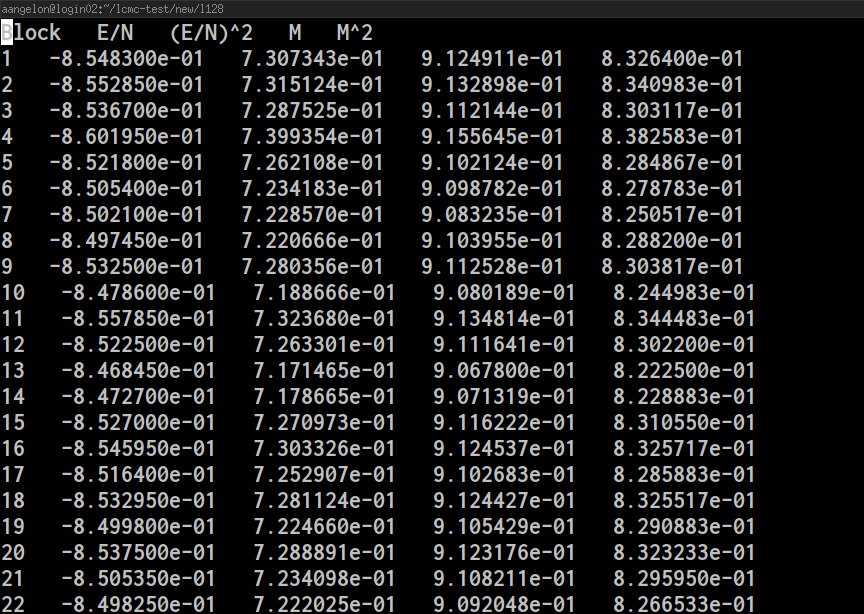
\includegraphics[width=0.55\textwidth]{pics/datafile.png}
    \end{center}

    Shell commands allow us to manipulate them as \focus{text files}:\\
    great versatility and relatively simple, sometimes requires attention

    You see files as a bunch of \focus{rows} or \focus{columns}:\\
    different commands for different tasks
  \end{center}
\end{frame}

\begin{frame}
  \begin{center}
    \frametitle{Row Operations I - Listing}

    \sidebyside{0.53}{
      \code{cat <file>} displays an entire file
      \begin{itemize}
        \item \code{-n}: numbers lines
      \end{itemize}
    }{\hfill}{0.44}{
      \begin{center}
        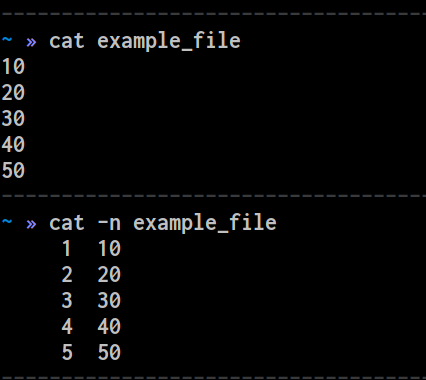
\includegraphics[width=0.50\textwidth]{pics/cat.png}
      \end{center}
    }

    \sidebyside{0.53}{
      \code{tail <file>}: \focus{last} 10 lines of the file
      \vspace{-4mm}
        \begin{itemize}
          \item \code{-n <num>}: last \code{<num>} lines
          \item \code{-n +<num>}: after line \code{<num>}
        \end{itemize}
      }{\hfill}{0.44}{
        \begin{center}
          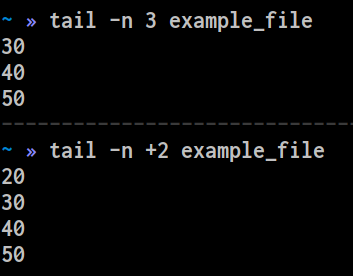
\includegraphics[width=0.50\textwidth]{pics/tail.png}
        \end{center}
      }

    \sidebyside{0.53}{
      \code{head <file>}: \focus{first} 10 lines of the file
      \vspace{-4mm}
        \begin{itemize}
          \item \code{-n <num>}: first \code{<num>} lines
          \item \code{-n -<num>}: before line \code{<num>}
        \end{itemize}
      }{\hfill}{0.44}{
        \begin{center}
          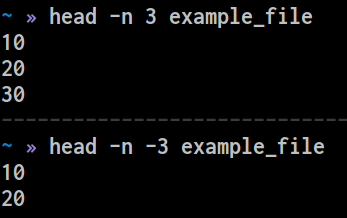
\includegraphics[width=0.50\textwidth]{pics/head.png}
        \end{center}
      }

      \vspace{4mm}

      Useful on their own, can be combined with \focus{pipes}
  \end{center}
\end{frame}

\begin{frame}
  \begin{center}
    \frametitle{Interlude I: Command piping}

    \sidebyside{0.60}{
      Output of a command \ra input to another\\
      (like water in a pipe)
    }{\hfill}{0.34}{
      \begin{center}
        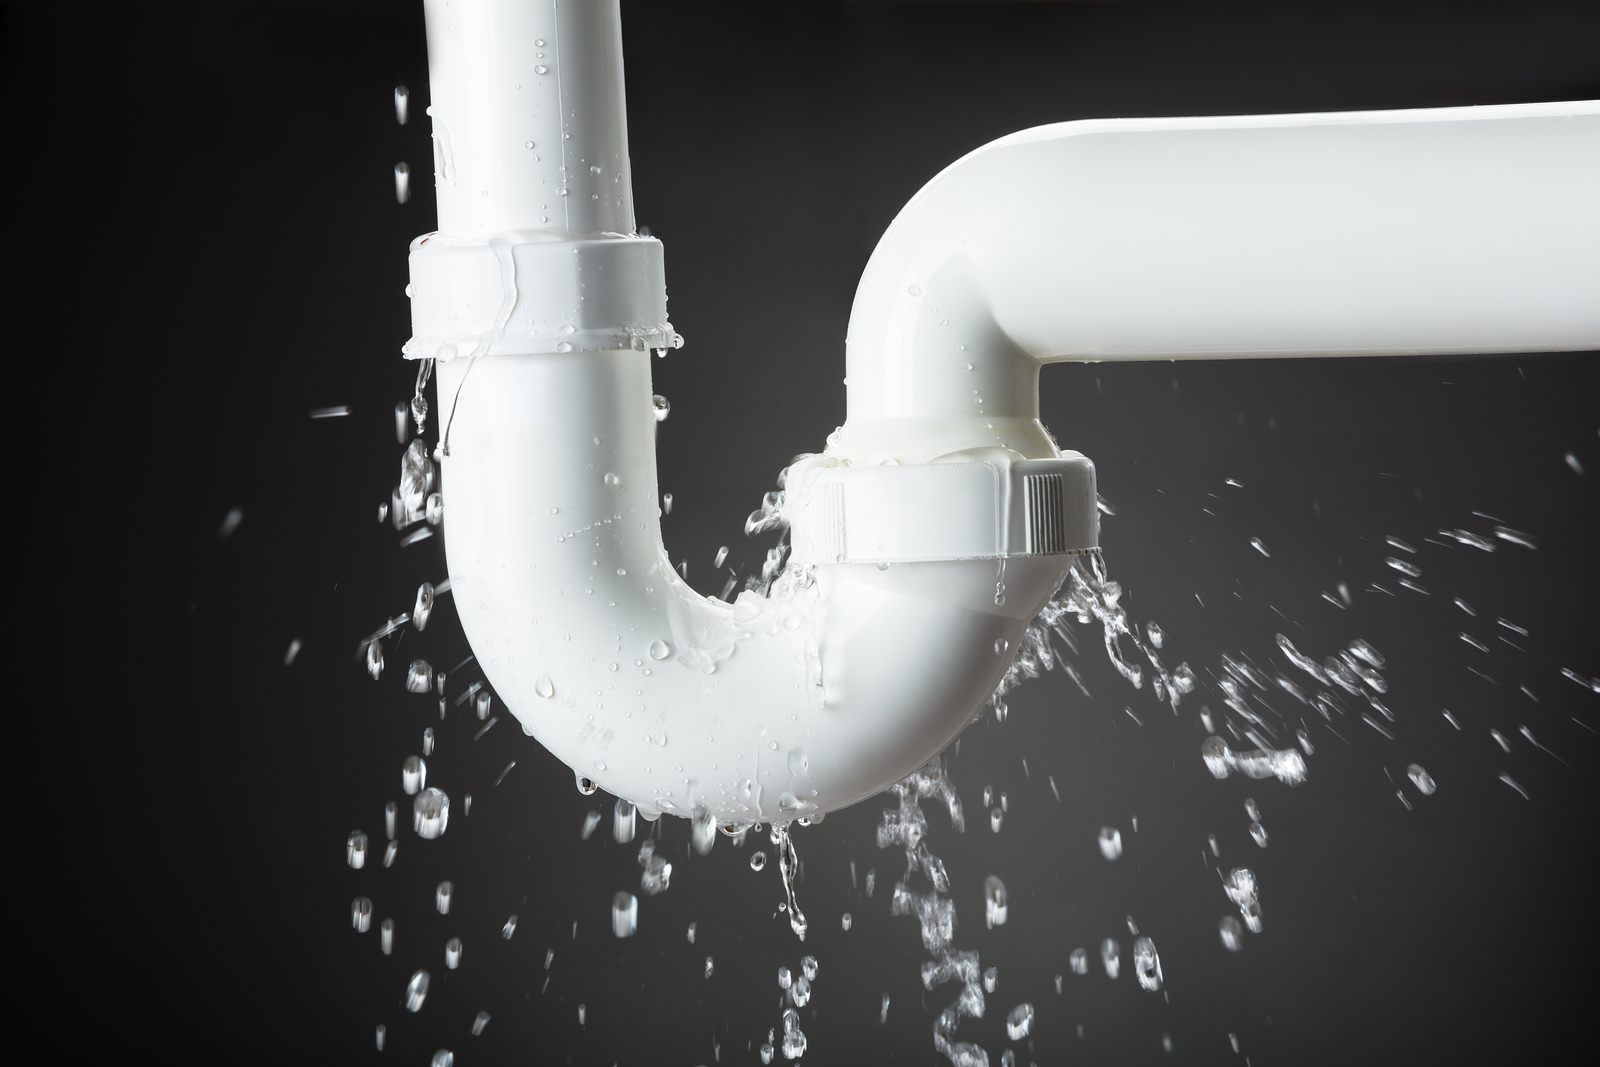
\includegraphics[width=1.00\textwidth]{pics/pipe.jpg}
      \end{center}
    }

    Syntax:
    \vspace{0.5mm}
    \code{command\_1 <arguments> | command\_2 | ... | command\_N}

    Trick: \focus{leftmost goes first}

    Example: extract 3rd line of file\\
    \code{head -n 3 file | tail -n 1}
  \end{center}
\end{frame}

\begin{frame}
  \begin{center}
    \frametitle{Row Operations II - Matching and Filtering}

    \code{grep <content> <files>} filters lines based on their content

    \sidebyside{0.59}{
      \begin{itemize}
        \item \code{<content>} can be a part of the line
        \item Quoting (\code{'<content>'}) is advised
        \item \code{-n}: adds numbers to matching lines
        \item \code{-i}: case-insensitive matching
        \item \code{-v}: prints non-matching lines
      \end{itemize}
    }{\hfill}{0.38}{
      \begin{center}
        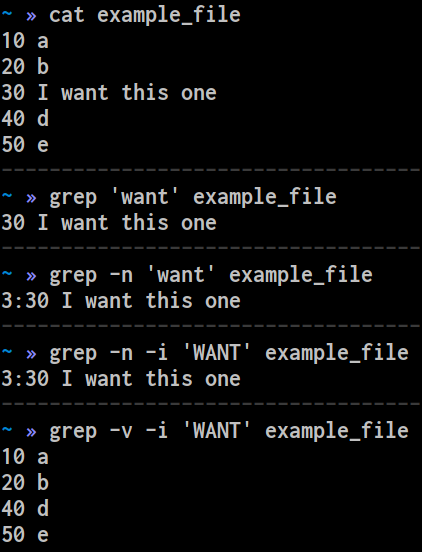
\includegraphics[width=1.00\textwidth]{pics/grep.png}
      \end{center}
    }

    More flexibility using \focus{regular expressions}
  \end{center}
\end{frame}

\begin{frame}
  \begin{center}
    \frametitle{Interlude II - Regular Expressions Basics}

    Regular expressions (regexps) are \focus{templates} that lines can match\\
    They can use special characters and \focus{wildcards}:

    \begin{itemize}
      \item \code{.}: any single character
      \item \code{.*}: any number of characters
      \item \code{\^}: beginning of the line
      \item \code{\$}: end of the line
      \item \code{[adf]}, \code{[a-z]}, \code{[A-Za-z]}: group of characters
    \end{itemize}

    Example: \code{The quick brown fox jumped}
    \vspace{-2mm}

    \begin{itemize}
      \item \code{.*quick.*} \green{matches}
      \item \code{The quick brown.*jumped.*} \green{matches}
      \item \code{The quick brown [foxape]* jumped .*} \green{matches}
      \item \code{\^{}quick.*} \red{doesn't match}
    \end{itemize}

    Now you can do \code{grep <regexp> <files>}:
    \code{grep '.*quick.*' <files>}
  \end{center}
\end{frame}

\begin{frame}
  \begin{center}
    \frametitle{Row Operations III - sed}

    \code{sed} (stream editor) operates on files as groups of lines:\\
    \focus{finds lines matching regexps and acts on (or around) them}

    \sidebyside{0.60}{
      \begin{itemize}
        \item \code{sed '/<regexp>/a <text>'}\\
          adds \code{<text>} after matching lines
        \item \code{sed '/<regexp>/i <text>'}\\
          adds \code{<text>} before matching lines
        \item \code{sed '/<regexp>/c <text>'}\\
          replaces matching lines with \code{<text>}
        \item \code{sed '/<regexp>/d'}\\
          deletes all matching lines
      \end{itemize}
    }{\hfill}{0.38}{
      \begin{center}
        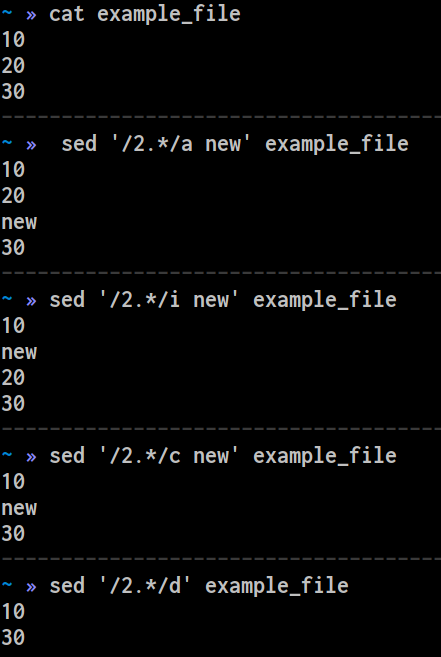
\includegraphics[width=1.00\textwidth]{pics/sed-1.png}
      \end{center}
    }
  \end{center}
\end{frame}

\begin{frame}
  \begin{center}
    \frametitle{Row Operations IV - More sed}

     \code{sed 's/<regexp>/<text>/g' <files>}\\
     replaces \focus{all} occurrence of \code{<regexp>} with \code{<text>} in all lines

   \sidebyside{0.54}{
     \begin{itemize}
        \item Replacement and matching\\
          will break words
        \item Matching is case-sensitive
        \item All regexp tools available
        \item \code{sed -i} applies modifications\\
          to the files: \focus{be careful!}
      \end{itemize}
    }{\hfill}{0.43}{
      \begin{center}
        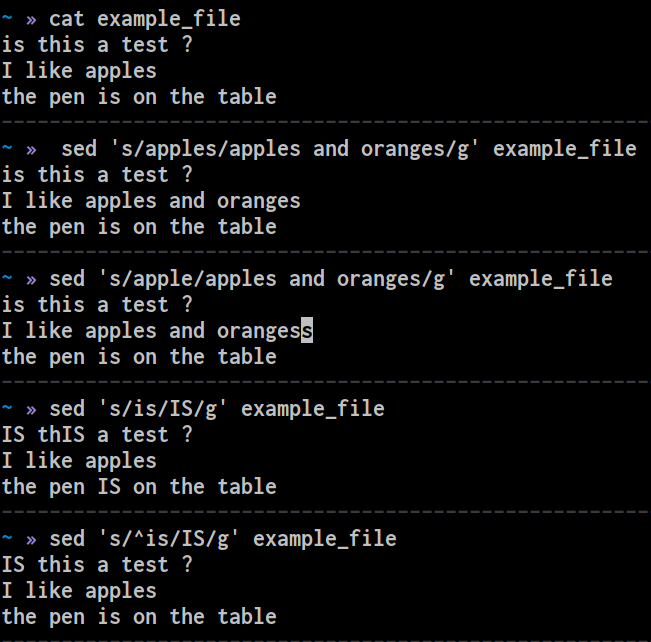
\includegraphics[width=1.00\textwidth]{pics/sed-2.png}
      \end{center}
    }

    Remember: \code{sed} can be used in pipes
  \end{center}
\end{frame}

\begin{frame}
  \begin{center}
    \frametitle{Column Operations I - cut and paste}

    Datafiles can also be seen as an ensemble of \focus{columns} (fields)

    \sidebyside{0.50}{
      \code{cut <options> <file>}:\\
      extract selected fields from file

      \begin{itemize}
        \item \code{-d}: specify field delimiter\\
          (often \code{' '} or \code{','})
        \item \code{-f}: specify the desired fields\\
          (separate with \code{,})
        \item \code{--complement}:\\
          print unselected fields
      \end{itemize}
    }{\hfill}{0.46}{
      \begin{center}
        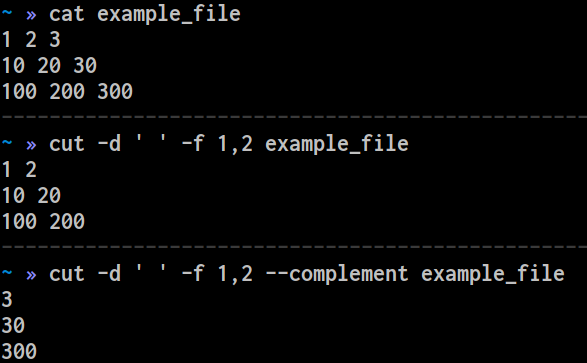
\includegraphics[width=1.00\textwidth]{pics/cut.png}
      \end{center}
    }

    \vspace{-4mm}

    \sidebyside{0.49}{
      \code{paste <files>}:\\
      join lines in multiple files
    }{\hfill}{0.48}{
      \begin{center}
        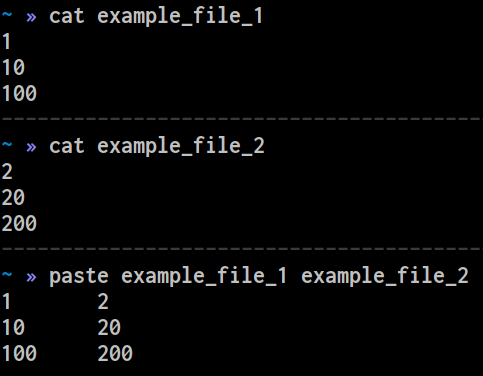
\includegraphics[width=0.75\textwidth]{pics/paste.png}
      \end{center}
    }

  \end{center}
\end{frame}

\end{document}
